\section{Problemløsning}

[Indledning til overafsnittet problemløsning]

\subsection{Teknologier til visualisering}
\label{sec:teknologianalyse}
Vi ser en tydelig mulighed for at assistere forbrugere med at træffe et valg, når det kommer til køb af varer på nettet. For at undersøge hvilke teknologier, der kan anvendes til visualisering, er der i dette afsnit en række teknologier og metoder, som alle er relevante i forhold til at visualisere en lampe. Teknologierne er udvalgt på baggrund af diskussion i gruppen, hvor mindre relevante teknologier, som f.eks. 3D-print blev fravalgt. Formålet med afsnittet er, at få en forståelse af hvilke teknologier der allerede eksisterer inden for visualisering, og finde ud af hvilke metoder, der er bedst i forhold til visualisering af lamper for brugere der handler via internettet.

\subsubsection{Digitale billeder taget med et fysisk kamera}
Som beskrevet under afsnit \ref{sec:ehandel}, benytter e-butikker, sig ofte af billeder til at vise kunden deres varer over internettet. Et eksempel på dette er vist på figur \ref{fig:e_handel_lampebilleder}.

\begin{figure}[H]
    \centering
    \fbox{\rule{\textwidth}{5cm}}
    \caption{Billeder af lamper på e-butikken somelampstore.what}
    \label{fig:e_handel_lampebilleder}
\end{figure} 

I det viste tilfælde er visualiseringen skabt ved at tage billeder af lamperne med et kamera fra en bestemt vinkel, i en kontekst, der typisk hænger sammen med lampetypen. 

Fordelen ved denne type af visualisering er, at den giver et virkelighedstro billede af, hvordan lampen ser ud i den kontekst, som billedet er taget i. \newline Ulempen er, at der ofte kun er et begrænset antal billeder til rådighed, hvilket kan medføre, at forbrugeren ikke kan se lampen fra alle vinkler og på den måde ikke kan visualisere lampen for sig. Derudover kan det være svært, at se hvordan lyset udbreder sig fra lampen, da dette til dels afhænger af hvilken vinkel man ser lampen fra. 

Herudfra kan man kortfattet sige, at visualisering af lamper gennem billeder, taget med et fysisk kamera, giver et realistisk billede af lampen, men kun i den kontekst og vinkel billedet er taget i. 

% \subsubsection{3D print}
% En teknologi, som lampebutikker vil kunne bruge, er 3D printere. 3D printere anvender plastik istedet for blæk, som bliver varmet op til knap 200 grader \cite{hvordan_3Dprinter}. Den flydende plastik bliver lagt i tynde lag og størkner hurtigt efter at have bundet sig med det underliggende lag. 

% Sælgeren kan give forbrugeren en fil, så forbrugeren selv vil være i stand til at lave et 3D print af en bestemt lampe. Dette forudsætter dog, at forbrugeren har en 3D printer og, at brugeren er dedikeret nok til at få printet lampen, da store objekter kan tage dage at printe og ofte skal deles op i mindre dele.\cite{hvordan_3Dprinter}. Derudover er 3D printere stadig en så ny teknologi, og de er stadig primært rettet mod hobbyfolk som vil bruge lang tid på, at få kallibreret printeren korrekt, da et print ellers nemt kan fejle. 3D printer er heller ikke en billig inverstering, da nogle modeller koster over titusinde kroner\cite{3D_printer}. 

% Idag vil det være en dårlig ide for lampebutikker at forvente, at deres kunder har en 3D printer derhjemme. Et andet problem er, at lampebutikker også kommer i et dilemma, da lampebutikker skal bestemme om man kan udgive tegninger inden forbrugeren har købt lampen eller om de skal betale en form for depositum.

\subsubsection{Computergrafik}
\label{sec:computergrafik}
I computergrafik, er en 3D model, en beskrivelse af objekters form og materiale.\cite{computergrafik_introduktion} Computergrafiske metoder kan bruges til at immitere hvordan lys interaktere med modellen og på den måde tegne et billede af modellen. Der eksisterer en mængde forskellige computergrafiske metoder, flere af hvilke kan bruges sammen med andre for, at opnå et mere realistisk eller effektivt resultat. Der findes flere produkter som kan visualisere produkter til salg på websites som f.eks. Cylindo\cite{Cylindo}. Men vi har ikke kendskab til at andre specialisere sig, eller markedsføre sig på nuværende tidspunkt med deres kompetencer med fokus på visualisering af lampers belysning.

\paragraph{Rasterisering}
er en metode til at visualisere miljøer med høj aktiv brugerinteraktion som f.eks. computerspil.\cite{rastarization} Metoden virker ved rent mattematisk at projektere modellen på et billedplan som repræsentere skærmen.\cite{rastarization}. Fordelen ved rasterisering er at disse projektioner, kan foretages meget hurtigt af computerens grafikkort, som bygget specielt til formålet\cite{rastarization}.\newline Ulempen er, at dette kan mindske fleksibiliteten, og muligheden for mere avancerede visualisering, hvor der kræves refleksioner og refraktioner af lys, som ikke passer ind i den proces (graphics pipeline\cite{rastarization}, som de enkelte grafikkort danner billeder ud fra. 

\paragraph{Ray tracing}\cite{raytracing_for_begyndere} forsøger, nøjagtigt at simulere lys i et virtuelt miljø, i modsætning til rasterisering hvor hastighed er den primære faktor. Raytracing bygger fundementalt på at følge stråler af lys og bygge en model for hvordan de stråler interagere med forskellige objekter og materialer. Der skælnes mellem to typer af raytracing: Forwards raytracing og backwards raytracing.

\subparagraph{Forwards raytracing}\cite{radiosity_by_wpi,radiosity_by_uob} er oftere kaldet radiosity og vil bliver reffereret til som sådan fremhenværende. Radiosity er hvad man kunne kalde en forwards raytracing metode. Her eksistere lyskilder ikke som specielle objekter i en 3D model, hvilket er tilfældet for de andre metoder, men her som objekter uden forskel fra de andre i modellen.

I radiosity modellen er alle flader betegnet med en absorbans faktor og en energi faktor. Absorbansen beskriver hvor meget af lys der rammer fladen der bliver absorberet. Absorberet lys hæver en flades energi og som i virkeligheden, afgives noget af den energi som lys, mens andet bliver omdannet til f.eks. varme. Lyskilder er således blot flader som starter med en mængde energi.

Radiosity er i stor grad blandt de mest tidskrævende metoder eftersom at den laver beregninger som ikke nødvendigvis bliver set i et billede. Dette muliggøre dog at visualisere en scene en gang og derefter at kunne se den fra mange vinkler eftersom at de ekstra udregninger allerede er gjort. Radiosity er derimod ikke designet til at håndtere fænomener som er afhængig af hvor man ser et objekt fra, så som refleksion og refraktion. Dvs. at radiosity ikke kan håndtere metalliske overflader eller semitransparente materialer. Til gengæld er Radiosity rigtig god til at simulere matte overflader og skygger.

\subparagraph{Backwards raytracing} er hvad man i almindelighed kalder raytracing og vil bliver reffereret til som sådan fremhenværende. Raytracing forsøger at simplificerer den fysiske model af lys ved at ignorere det lys som ikke rammer vores øjne. Raytracing er dog alligevel blandt de metoder som kendes for at kunne skabe de mest fotorealistiske renderinger. Dette gøres ved såkaldt \textit{backwards raytracing}, hvorved man følger en stråle fra øjet og ud mod 3D modellen, så tjekkes der for kollisioner mellem strålen og objekterne i modellen. Ved hver kollision kan man vælge at følge yderligere stråler som kan hjælpe med at udregne refleksioner eller komplekse skygger. Denne metoder står i modsætning til hvad man kalder \textit{forwards raytracing} som er den mere fysisk korrekte metode, hvor man følger stråler af lys fra hver lyskilde.

I forhold til rasterisering, tager raytracede billeder væsentligt længere tid at tegne, men komplekse lysfænomener som refleksioner og lys forvrængninger igennem semitransparante medier som vand(kaldet refraktion) er simple at beskrive for en raytracing algoritme, som kan tegne disse med realistisk precision. Nogle fænomener som bløde skygger kan også beskrives men jo flere typer fænomener og jo større realisme der kræves des længere tid tager det at tegne et billede, men raytracing tillader stor fleksibilitet.

\subsubsection{Augmented Reality App}

Augmented Reality er en teknologi der kan sætte virtuelle objekter ind i en virkelig kontekst. Derudover har man mulighed for at interagere med objektet i real tid. 
Denne metode bruger producenten "Artemides" i deres Augmented Reality App. Appen virker ved, at man scanner et logo fra et fysisk lampekatalog, hvorefter en givet lampe vil vise sig på logoets plads. Det er herefter muligt at flytte kataloget for, at se lampen i forskellige kontekster. Derudover har man mulighed for at rotere i alle vinkler samt tænde og slukke for lampens pære. 
Fordelene ved appen er, at brugeren har mulighed for selv at vælge hvilken lampe de vil se i sin egen kontekst, samt interagere med lampen. Herved har brugeren mulighed for, at se præcist hvordan lampen ser ud. 
Ulemperne ved appen er, at den ikke visualisere lampens belysning særlig godt, da dens første priotet er at visualisere selve lampens design. Derudover er det ikke muligt at visualisere lamper i en kontekst, hvis man ikke har den nødvendige bog som indeholder logoer over de forskellige lampedesigns i 3D. En anden ulempe er, at lampeudvalget er meget begrænset da det kun er udvalgte produkter fra "Artemides" som kan visualiseres. 
Nedenstående figur viser "Artemides" brugervejledning til appen.

\begin{figure}[H]
    \centering
    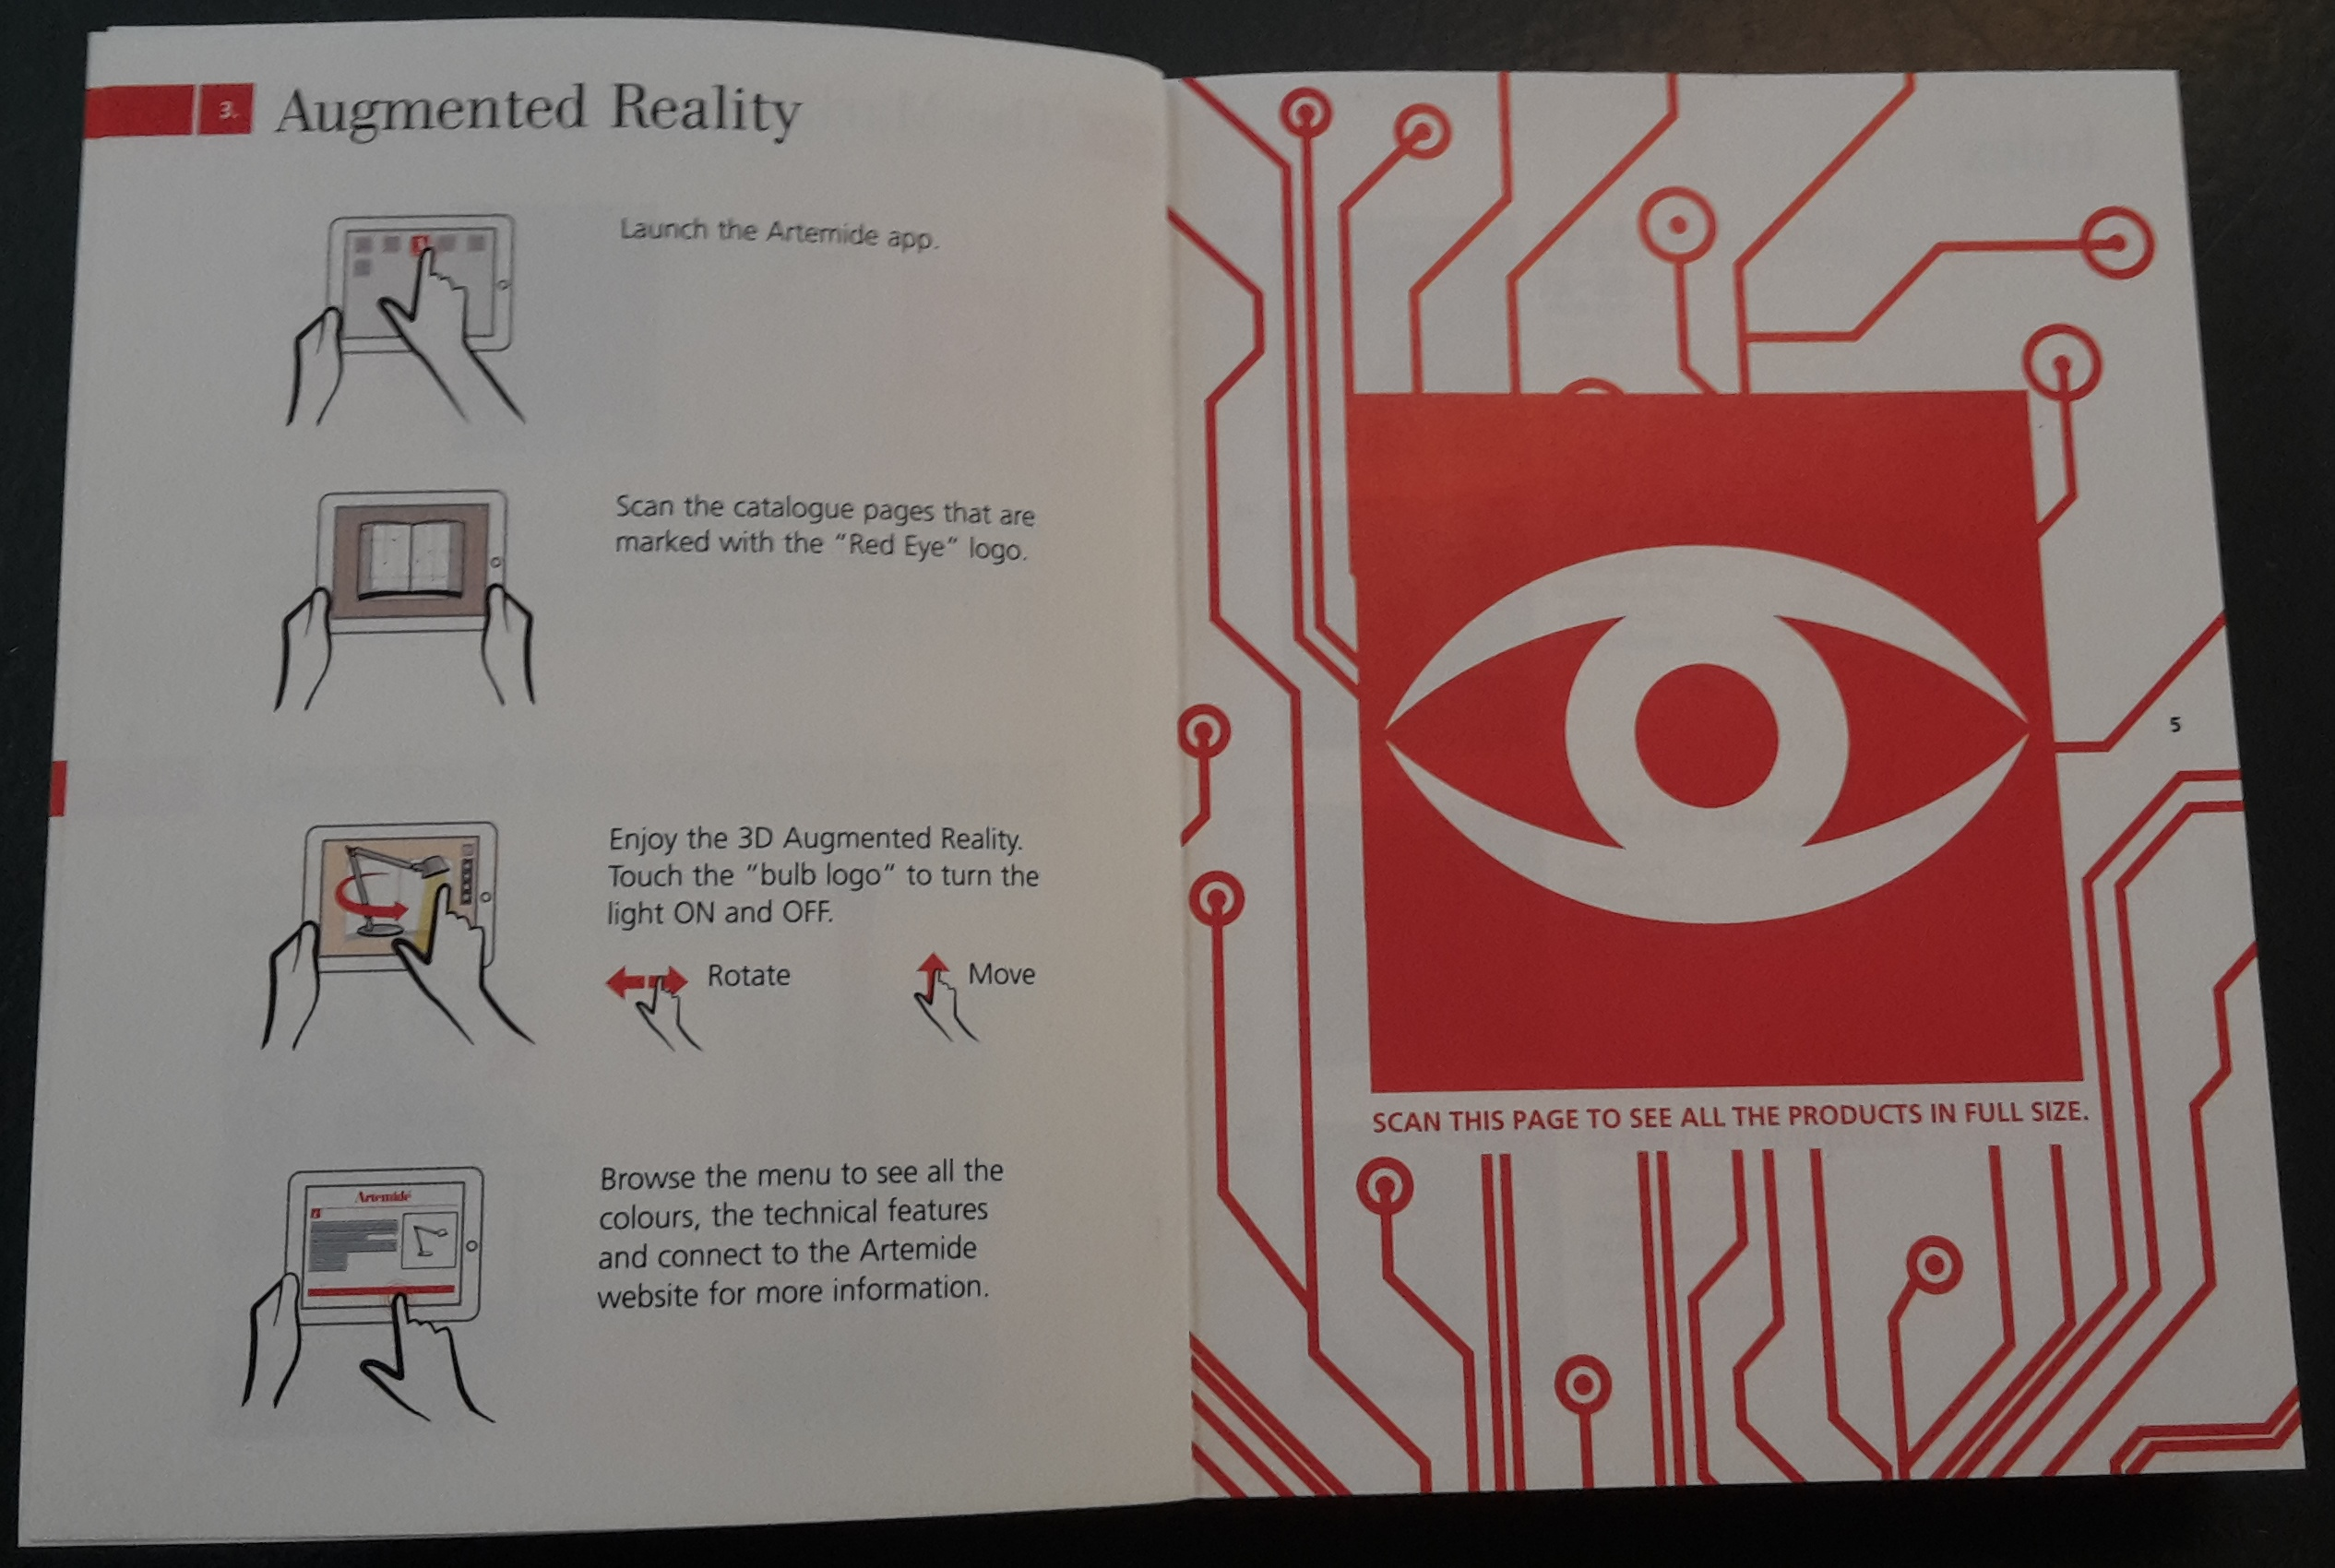
\includegraphics[width=10cm]{augmented_reality_artemides}
    \caption{Brugervejledning fra Artemides augmented reality.}
    \label{fig:augmented_reality_artemides}
\end{figure} 


\subsubsection*{Opsummering}
Billeder af den fysiske lampe er gode til akkurat at gengive lampen, men det er et problem at der ofte ikke er billeder nok fra forskellige vinkler, at billederne kun viser lampens form og ikke dens lys og at det er for besværligt at tage billeder af lampen med forskellige pærer for at vise forskellige farvetemperature og at det også er bbesværligt at udskifte den kontekst som lampen bliver vist i. 

Computergrafik kan nemt indlejres i en hjemmeside. Hvilken Computergrafisk teknik der er den korrekte er et case til case valg eftersom det helt afhænger af hvor meget fleksibilitet versus kvalitet der er nødvendigt. Rasterisering og radiosity kan begge implementeres på en måde hvorved der opnås et højt niveau af bruger interaktion som kan gøre værktøjet mere naturligt at anvende for forbrugeren. Eftersom at målet er at simulere lamper og ikke møbler som borde og stole, er langt mere komplekst at lave en god visualisation med rasterisering. Radiosity falder også til kort hvis der er behov for mere komplekse materialer som metalliske overflader eller f.eks. klar plast og glas. Billeder tegnet med raytracing kan tage lang tid at rendere, men der er mulighed for stor fleksibilitet og komplekse materialer er relativt simple at rendere. Med det grundlag vil rapporten fremadrettet arbejde med raytracing som metode til visualisering.

\subsection{Ide}

\subsection{Teknologier til visualisering}
\label{sec:tek_til_visualisering}
Vi ser en tydelig mulighed for at assistere forbrugere med at træffe et valg, når det kommer til køb af varer på nettet. Formålet med afsnittet er, at få en forståelse af hvilke teknologier der allerede eksisterer inden for visualisering, og finde ud af hvilken teknologi, der er bedst i forhold til visualisering af lamper for kunder, der besøger en e-butiks hjemmeside. De enkelte teknologier vurderes på baggrund af de krav, der er sat til løsningsforslaget i afsnit \ref{sec:losning}.

\subsubsection{Digitale billeder taget med et fysisk kamera}
Som beskrevet under afsnit \ref{sec:ehandel}, benytter e-butikker, sig ofte af billeder til at vise kunden deres varer over internettet. Et eksempel på dette er vist på figur \ref{fig:e_handel_lampebilleder}.

\begin{figure}[H]
    \centering
    \fbox{\rule{\textwidth}{5cm}}
    \caption{Billeder af lamper på e-butikken somelampstore.what}
    \label{fig:e_handel_lampebilleder}
\end{figure} 

I det viste tilfælde er visualiseringen skabt ved at tage billeder af lamperne med et kamera fra en bestemt vinkel, i en kontekst, der typisk hænger sammen med lampetypen. 

Fordelen ved denne type af visualisering er, at den giver et virkelighedstro billede af, hvordan lampen ser ud i den kontekst, som billedet er taget i. Ulempen er, at der ofte kun er et begrænset antal billeder til rådighed, hvilket kan medføre, at forbrugeren ikke kan se lampen fra alle vinkler og på den måde ikke kan visualisere lampen for sig. Derudover kan det være svært, at se hvordan lyset udbreder sig fra lampen, da dette til dels afhænger af hvilken vinkel man ser lampen fra. 

Herudfra kan man kortfattet sige, at visualisering af lamper gennem billeder, taget med et fysisk kamera, giver et realistisk billede af lampen, men kun i den kontekst og vinkel billedet er taget i. 


\subsubsection{Computergrafik}
\label{sec:computergrafik}
I computergrafik, er en 3D model, en beskrivelse af objekters form og materiale \cite{computergrafik_introduktion}. Computergrafiske metoder kan bruges til at simulere, hvordan lys interagere med modellen og på den måde tegne et billede af modellen. Der eksisterer forskellige computergrafiske metoder, flere af hvilke kan bruges sammen med andre for, at opnå et mere realistisk eller effektivt resultat. Der er allerede værktøjer, som kan visualisere produkter til salg på websites som f.eks.\ Cylindo \cite{Cylindo}. Vi har ikke kendskab til at andre specialiserer sig, eller markedsfører sig på nuværende tidspunkt med deres kompetencer med fokus på visualisering af lampers belysning. Derfor er der herunder beskrivelse af to af de mest anvende metoder inden for computergrafik.

\paragraph{Rasterisering}
er en metode til at visualisere miljøer med høj aktiv brugerinteraktion som f.eks.\ computerspil \cite{rastarization}. Metoden virker ved rent matematisk at projektere modellen på et billedplan som repræsentere skærmen \cite{rastarization}. Fordelen ved rasterisering er at disse projektioner, kan foretages meget hurtigt af computerens grafikkort, som er bygget specielt til formålet \cite{rastarization}. Dette kan dog mindske fleksibiliteten, og muligheden for mere avancerede visualisering, hvor der kræves refleksioner og refraktioner af lys, som ikke passer ind i den proces (graphics pipeline \cite{rastarization}, som de enkelte grafikkort danner billeder ud fra). 

\paragraph{Ray tracing} [DER MANGLER KILDER TIL PÅSTANDE I DETTE AFSNIT]() forsøger, nøjagtigt at simulere lys i et virtuelt miljø, i modsætning til rasterisering hvor hastighed er den primære faktor. Raytracing bygger fundamentalt på at følge lysstråler og bygge en model for hvordan lysstrålerne interagere med forskellige objekter og materialer \cite{raytracing_for_begyndere}. 

I forhold til rasterisering, tager det længere tid at tegne, men komplekse lysfænomener som refleksioner og lys forvrængninger igennem semitransparante medier som vand(kaldet refraktion) er simple at beskrive for en raytracing algoritme, som kan tegne disse med realistisk precision. Nogle fænomener som bløde skygger kan også beskrives men jo flere typer fænomener og jo større realisme der kræves des længere tid tager det at tegne et billede, men raytracing tillader stor fleksibilitet.

\subsubsection{Augmented Reality}
Der er nu blevet gennemgået visualisering af virkelige objekter ved hjælp af digitale billeder og virtuelle objekter ved hjælp af computergrafik. I dette afsnit beskrives augmented reality som er en teknologi der kombinerer virkelige og virtuelle objekter \cite{augmented_reality}.

Augmented reality fungerer ved at tage et billede med et normalt kamera, og herefter ændrer billedet ved at indsætte computergrafik på billedet \cite{augmented_reality}.

Et eksempel på anvendelsen af augmented reality er Artemides Augmented Reality App. Denne app gør det muligt, at visualisere udvalgte lamper i en kontekst som brugeren selv vælger \cite{artemides}. 

Fordelen ved augmented reality i forhold til løsningsforslaget er, at den muliggøre at se lampen fra flere forskellige vinkler i den kontekst som kunden ønsker. Hvis der ses bort fra tekniske udfordringer så ville det også være en fordel hvis kunden kunne visualisere en lampe og dens belysning i den kontekst som kunden ønsker at købe lampen til. \newline Ulempen ved augmented reality i forhold til løsningsforslaget er, at det er en teknisk udfordring, at få en rummelig forståelse for den virkelig kontekst så det virtuelle der indsættes får en tilstrækkelig realisme. Det vil derfor være svært at simulere lampens belysning hvis man ikke kender til dimensioner eller materialerne i den virkelige kontekst. Hvis det lykkedes, at få en forståelse for de virkelige objekter i billedet, så vil det stadigvæk være raytracing eller en anden teknik indenfor computergrafik som ville være at foretrække når man skal visualisere lampens belysning. Derfor er udfordringen ved augmented reality dobbelt, da den både skal få en rummelig forståelse for de virkelige objekter i billedet, samt lave en realistisk computergrafik som passer ind i billedet.



\subsubsection*{Opsummering}
Ud fra ovenstående afsnit er der udledt følgende fordele og ulemper for de enkelte teknologier.
\begin{table}[H]
  \centering
  
\center
    \begin{tabular}{ | p{3cm} | p{5cm} | p{5cm} |}
    
    \hline
    Teknologi & Fordele & Ulemper \\ \hline
    Kamerabilleder & Realistisk visualisering. & Tidskrævende. Begrænset kombinationer af lampen, synsvinkel, farvetemperatur og kontekst. \\ \hline
   Computergrafik & Nemt at integrere på lampebtuikker hjemmesider. Kan opnå høj realisme af lampen og dens belysning. \newline Nemt at ændre vinkel, farvetemperatur og kontekst hvorfra lampen visualiseres. & Kræver 3D-model af lampen og konteksten. Kræver meget computerkraft ved høj realisme. \\ \hline
   Augmented Reality & Lampen kan visualiseres fra flere vinkler og i den kontekst som kunden ønsker at købe lampen til. & Det er en teknisk udfordring at virtuelle objekter med den virkelige kontekst, så der stadigvæk opnås en hvis realisme. \\ \hline
    \end{tabular}
  \caption{Viser fordele og ulemper ved de tre teknologier til visualisering.}
\label{tab:fordele_ulemper_teknologier}
\end{table}

På baggrund af fordele og ulemper vist i tabel \ref{tab:fordele_ulemper_teknologier} sammenlignes de tre teknologier nu med de krav, der er opstillet til løsningsforslaget i afsnit \ref{sec:losning}. 

Billeder af fysiske lamper taget med et kamera, kan bidrage til udviklingen af løsningsforslaget, da den delvist opfylder krav 1-3 og 5. Da det er muligt at tage et billede af lampen og dens belysning med en bestemt farvetemperatur og fra en bestemt vinkel. Derudover kan løsningen implementeres på en e-butikshjemmeside, ved blot at bruge de billeder, der tages med kameraet. Ulempen er, at det kan være ressourcekrævende, da der skal tages billeder med forskellige lamper, farvetemperaturer og vinkler som giver mange kombinationer og dermed mange billeder.

Hvordan computergrafik kan biddrage med at løse kravene i afsnit \ref{sec:losning}, afhænger af hvilken teknik man benytter. Hvis man benytter rasterisering, vil det være svært at opfylde krav 1, da visualisering af lampens belysning kræver, at der anvendes lysfænomener, som ikke passer ind i modellen for rasterisering. Rasterisering vil dog være oplagt til at opfylde krav 2 og 4, da den som nævnt er bygget til at rendere et billede med høj brugerinteraktion og kort renderingstid.
Raytracing vil derimod være oplagt til at opfylde krav 1-3, da det er muligt at simulere lampen og dens belysning med forskellige farvetemperaturer og vinkler. Derudover kan raytracing implementeres i løsningen, der renderer et billede, der kan vises på en e-butikshjemmeside, hvilket gør at den opfylder krav 5. Ulempen ved raytracing er, at det kan være svært at opfylde krav 4, da simulering af lampens belysning kan være en tidskrævende proces.

Augmented reality kan bidrage til udviklingen af løsningsforslaget ved at den har potentialet for at opfylde de samme krav, som både visualisering vha.\ kamerabilleder og computergrafik (krav 1-3). Dog er dette en teknisk udfordring, da den rummelige forståelse af den virkelige kontekst af billedet er nødvendig for at kunne opnå en realistisk visualisering, når computergrafikken indsættes. I forhold til krav 4 har augmented reality den samme udfordring som f.eks.\ raytracing, da simulering af lampens belysning kan være en tidskrævende proces. Derudover kan det være svært at implementere augmented reality på en e-butikshjemmeside, da det kræver adgang til kundens kamera. Ud fra ovenstående har vi valgt raytracing som teknologi til visualisering, da den har potentialet for at opfylde kravene opstillet i afsnit \ref{sec:losning}, uden at være en lige så stor teknisk udfordring som augmented reality. 


\clearpage



\subsection{Ide}

I dette afsnit er der beskrevet en ide til løsningen af den endelige problemformulering. Ideen er resultatet af en diskussion i gruppen, hvor vi kom med ideer til løsninger, og herefter diskuterede fordele og ulemper ved de forskellige ideer. Formålet med afsnittet er at skitsere gruppens bud på den optimale løsning på problemet, og afsnittet er derfor udarbejdet med feedback fra forskellige lampebutikker. I slutningen af afsnittet vil der være en afgrænsning af løsningen som vil danne grundlag for den senere udvikling af en løsning.

Den løsning som gruppen har valgt at arbejde med er, "3D modeller af lamper med interaktion". Som beskrevet i problemanalysen har gruppen valgt at løse problemet når kunder handler på e-butikker. Tanken er derfor at implementere software på en e-butiks hjemmeside med henblik på at løse problemet for kunden.

\subsubsection{Skitse af løsning}

\begin{figure}[H]
   \centering
   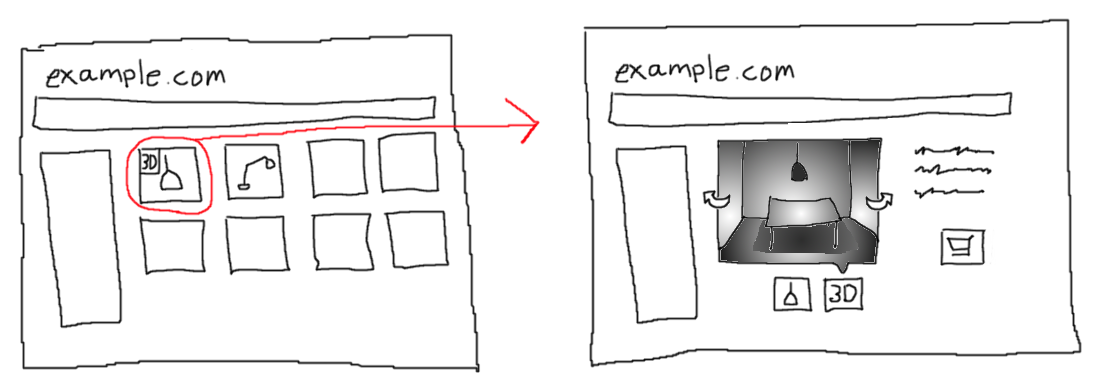
\includegraphics[width=\textwidth]{skitse_til_loesning}
   \caption{Skitse af ide til løsning.}
\end{figure}

På figur 5 er der illusteret en skitse af en e-butik som sælger lamper. Figuren illustrerer hvordan systemet kan integreres på en hjemmeside. Skitse 5a viser et online katalog over e-butikkens udvalg af lamper. Som der fremgår af skitsen vil nogle lamper være markeret med et "3D-ikon" og dette indikerer, at kunden har mulighed for, at se skitsen i 3D. Kunden tilgår 3D-billedet ved at klikke på ikonet. Når kunden trykker på ikonet bliver kunden omdirigeret til en anden menu. Som der fremgår af skitse 5b, så har kunden her mulighed for at se en 3D-model af lampen i et rum. De to pile på skitsen indikerer, at kunden har mulighed for at rotere billedet, og se hvordan belysningen fra lampen er, set fra forskellige vinkler. Som en ekstra feature har kunden mulighed for at indtaste en kontekst, beskrevet som en model, ind i programmet og har derefter mulighed for at se hvordan lampen ser ud i den kontekst som kunden ønsker. 
Derudover har kunden mulighed for, at justere lampens farvetemperatur (i kelvin), meningen med denne feature er, at kunden har mulighed for at visualisere hvordan forskellige pærer vil se ud i lampen. De forskellige 3D billeder vil ligge til rådighed på en ekstern server og vil derfor ikke gøre e-butikkernes hjemmeside betydeligt langsommere. Derudover er tanken af alle 3D billeder bliver udleveret af producenten af lamperne. 

\begin{figure}[H]
   \centering
   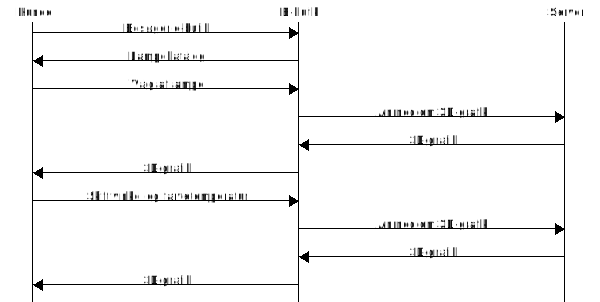
\includegraphics[width=\textwidth]{brugerinteraktion}
   \caption{Sekvensdiagram af løsningsideen.}
\end{figure}

Figur 6 tager udgangspunkt i en hjemmeside som har fået implementeret vores løsning, og viser et sekvensdiagram som illustrere processen når en kunde vil købe en lampe.  

I forbindelse med implementeringen af softwaren på en hjemmeside har der været forskellige ting som skulle overvejes. Da problemet omhandler visualisering af lys fra lamper, har gruppen valgt at fokusere på at lave en løsning hvis primære formål er at generere realistiske 3D-billeder af lamper. Disse billeder vil vise belysningen fra lamper med forskellige pærer. Features som interaktion og kontekst, har derfor anden priotet. 

Ud fra ovenstående beskrivelse har gruppen derfor valgt, i første omgang, at fokusere på at lave et program der gør det muligt for kunden, at visualisere hvordan lys spreder sig fra lamper illustreret igennem realistiske 3D-billeder. Derudover har kunden mulighed for at justere pærens farvetemperatur, og derved også se hvordan lampens belysning med forskellige pærer.  


\subsubsection{Krav til løsningen}

I forbindelse af vores projekt har vi fået nogle krav fra universitetets side. Disse er at programmet skal skrives i programmeringssproget C, derudover er der også tidsmæssigt pres da hele projektet kun varer ca.\ to en halv måned. 
Vi er også begrænset af vores egen viden indenfor emnet, da raytracing er en fremmed teknik, som få af os har haft tidligere erfaringer med. 

Vi har selv opstillet nogle krav til vores program for hvad vi mener programmet skal kunne før det kan være et færdigt produkt.
\begin{enumerate}
    \item Programmet skal kunne implementeres på en hjemmesiden (ellers bruges på en computer i den fysiske butik).
    \item skal kunne visualisere billedet relativt hurtigt, da kunderne ikke skal vente før de kan se billedet.
    \item Programmet skal kunne modtage et vilkårligt billede (i den rigtige format) og renderer dette.
    \item Lysets udbreddelse skal kunne ses tydeligt af kunden.
    \item Det skal være muligt for kunden skal kunne ændre farvetemperatur.
    \item Det skal være muligt for kunden at rotere billedet.
    \item Det skal være muligt for kunden at kunne indsætte en vilkårlig kontekst.
    \item Programmet skal være let at bruge, så en potentiel kunde ikke vil blive frusteret og derved vil forlade butikken/siden.
    \item 
\end{enumerate}

\subsubsection*{Opsummering}
[Kort opsummering af præcist ideen bag løsningen]

\subsection{Teori}
\label{sec:teori}

Dette afsnit omhandler de teorier samt videnskabelige principper som er relevante i forhold til at lave den løsning som er beskrevet i afsnit \ref{sec:losning}. Der vil derfor i afsnittet være fokus på de principper, formler og algoritmer som der bruges i udviklingsfasen. Teoriafsnittet vil primært fokusere på at beskrive og undersøge tekniske og matematiske principper som ellers ville være svære at forstå og arbejde med. Ud fra kravene til løsningen i afsnit \ref{sec:krav} har gruppen valgt at undersøge og diskutere følgende fænomener og principper: Rotationsmatricer i afsnit \ref{sec:rot_matricer}, konvertering af farvetemperatur til RGB-værdier i afsnit \ref{sec:temptilrgb}, fra 3D-model til billede i afsnit \ref{sec:fra_model_til_billede} herunder 3D-model, kamera, perspektiv projektion, backwards raytracing, phong-modellen og til sidst skæring mellem linje og trekant i rummet i afsnit \ref{sec:triangle_intersection}. I slutningen af afsnittet vil der fremgå, hvordan de enkelte teorier kan bidrage til udviklingen af løsningen.

\subsubsection{Rotationsmatricer}
\label{sec:rot_matricer}
Hvis vi vil rotere et punkt eller en vektor omkring nul-punktet i et koordinatsystem kan vi bruge en rotationsmatrix \cite{rotationsmatricer}.
En rotationsmatrix er en matrix, der, hvis multipliceret sammen med en anden matrix, roterer en vektor eller et punkt i et koordinatsystem.
\begin{align} \label{eu_eqn}
  R_x(\theta) = 
  \begin{bmatrix}
  \label{eq:rotate_around_x}
    1 & 0 & 0\\ 
    0 & cos \theta & - sin \theta\\ 
    0 & sin \theta & cos \theta
  \end{bmatrix}\\
    R_y(\theta) =
  \begin{bmatrix}
    cos \theta  & 0 & sin \theta\\ 
    0           & 1 & 0\\ 
    -sin \theta & 0 & cos \theta
  \end{bmatrix}\\
    R_z(\theta) = 
  \begin{bmatrix}
    cos \theta & - sin \theta & 0\\ 
    sin \theta & cos \theta & 0\\
    0 & 0 & 1
  \end{bmatrix}
\end{align}
Vi indsætter den vinkel som vi vil dreje vektoren med i radianer og multiplicerer dem sammen som angivet i udtryk \ref{eq:rotate_around_x}. Vektoren bliver drejet omkring nul-punktet med netop den mængde radianer, som er angivet.
Nedenstående eksempel illustrerer princippet ved at dreje en vektor i rummet.

\begin{equation}
  {\vv{u}} =
  \begin{bmatrix}
    u_x \\ 
    u_y \\
    u_z
  \end{bmatrix}
\end{equation}
og rotationsvektor \begin{math}R_x\end{math}
\begin{equation}
  R_x(\theta) = 
  \begin{bmatrix}
    1 & 0 & 0\\ 
    0 & cos \theta & - sin \theta\\ 
    0 & sin \theta & cos \theta
  \end{bmatrix}
\end{equation}
Den roterede vektor $\vv{u}$ kan nu beskrives som set i udtryk \ref{eq:rotation_x}
\begin{equation}
  \vv{v} = R_x(\theta) \cdot \vv{u} = \begin{bmatrix}
    u_x \\ 
    cos(\theta)   \cdot u_y - sin(\theta) \cdot u_z \\
    sin(\theta) \cdot u_y + cos(\theta) \cdot u_z
  \end{bmatrix}
  \label{eq:rotation_x}
\end{equation}
Og kalder det for vektor $\vv{v}$ og indsætter både $\vv{u}$ og $\vv{v}$ i nedenstående skitse.
\begin{figure}[H]
  \center
  \begin{tikzpicture}
    \coordinate (O) at (0,0) ;
    \coordinate (u) at (2, 1) ;
    \coordinate (v) at (1, 2) ;

    \draw[thick,->] (O) -- (4.5,0);
    \draw[thick,->] (O) -- (0,4.5);
    \draw[thick,->] (O) -- (4.5,0) node[anchor=north west] {y};
    \draw[thick,->] (O) -- (0,4.5) node[anchor=south east] {z};

    \draw [blue!50, thick, -{Stealth[width=3mm, length=3mm]}] (O) -- (u);
    \draw [blue!50, thick, -{Stealth[width=3mm, length=3mm]}] (O) -- (v);
    \node [below right] at (u) {$u$};
    \node [below] at (v) {$v$};
    \draw (1, 1) arc (10:10:1);
    \node[] at (1,1.2)  {$\theta$};
  \end{tikzpicture}
  % 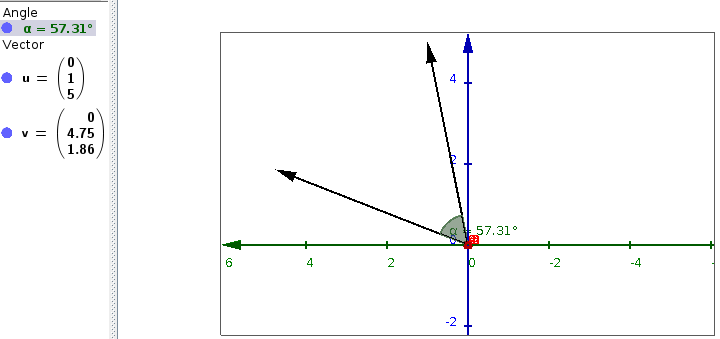
\includegraphics[width=12cm]{rotationsmatrix_eksempel.png}
  \caption{Eksempel på en rotationsmatrix}
  \label{fig:rotationsmatrix_eksempel}
\end{figure}
% Geogebra udregner vinkler i grader, så vi omregner grader til radianer ved hjælp af ligningen:
% \begin{equation}
  % R=d/2*\pi/360=57,31/2*\pi/360\approx1
% \end{equation}
Vi ser at vektor $\vv{u}$ blev drejet \theta radianer, som forventet.


\subsubsection{Konvertering fra farvetemperatur til RGB}
\label{sec:temptilrgb}
Farvetemperatur, som også er beskrevet nederst i \ref{sec:lys}, er temperaturen af et udsendt lys og måles i kelvin. Denne temperatur kan bruges til at finde ud af, om et lys er varmt eller koldt. 
RGB-værdien er en værdi for en given farves indhold af rød, grøn og blå. Værdien angives normalt ved et tal mellem 0 og 255, altså er RBG-værdien [0, 128, 255] ingen del rød, en del grøn og fuld blå, hvilket, blandet sammen, giver en blålig farve.
Der findes ingen direkte og 100\% præcis formel for at ’oversætte’ en kelvintemperaturværdi til en RGB-værdi, derfor har rapporten taget udgangspunkt i en algoritme, som er lavet ud fra 400 målinger, men som stadig ikke er præcis nok til videnskabelig brug \cite{tanner_helland}.
Måden hvorpå algoritmen er lavet, er ved at tage disse 400 målinger, og lave en funktion ud fra dem. Der er lavet én måling per 100 kelvin, der starter ved 1000 kelvin og slutter ved 40.000 kelvin \cite{charity_values}. Ved at kigge på funktionen \cite{tanner_helland_chart} har Tanner Helland kunne konkludere  tre ting:

\begin{itemize}
\item Røde værdier under 6600 kelvin er altid 255.
\item Blå værdier under 2000 kelvin er altid 0.
\item Blå værdier over 6500 kelvin er altid 255.
\end{itemize}

Disse tre, forholdsvis simple, konklusioner har hjulpet med at gøre algoritmen meget kortere og mere simpel. Herunder kan udregningerne for hhv\.  rød-, grøn- og blå-værdierne ses matematisk, før de er skrevet om til kode. Matematikken er vist gennem gaffelfunktioner, altså funktioner med forskellige funktionsudtryk for bestemte intervaller.


\begin{displaymath}
   R(k) = \left\{
     \begin{array}{lr}
       255 &1000 <= \text{k $\land$ k} <= 6600\\
       329.698727446*(k-60^{-0.1332047592}) &6600 < \text{k $\land$ k} <= 40000
     \end{array}
   \right.
\end{displaymath} 

\begin{displaymath}
   G(k) = \left\{
     \begin{array}{lr}
       99.4708025861*\ln(k)-161.1195681661 &1000 <= \text{k $\land$ k} <= 6600\\
       288.1221695283*(k-60^{-0.0755148492}) &6600 < \text{k $\land$ k} <= 40000
     \end{array}
   \right.
\end{displaymath} 

\begin{displaymath}
   B(k) = \left\{
     \begin{array}{lr}
       255 &6600 <= \text{k $\land$ k} <= 40000\\
       0 &1000 <= \text{k $\land$ k} <= 1900\\
       138.5177312231 * \ln(k-10) - 305.0447927307 &1900 < \text{k $\land$ k} < 6600
     \end{array}
   \right.
\end{displaymath} 

Grunden til at der oversættes fra farvetemperatur til RGB-værdi, er for at kunne visualisere farverne på en computer. Et billede vist på en computer består af pixels, som alle har en RGB-værdi, derfor kan lyset fra en lampe med en given farvetemperatur visualiseres, hvis farvetemperaturen oversættes til RGB-værdi.

\paragraph*{Opsummering}
Vi har nu set hvordan man kan konvertere en farvetemperatur i Kelvin til RGB-værdier. Derudover har vi set, hvordan man kan rotere en vektor ved hjælp af matricer. Denne viden er nødvendig for at kunne opfylde kravene om at løsningen skal gøre det muligt at vise lampen med forskellige farvetemperaturer og vinkler. 











\subsubsection{Fra 3D-model til billede}
\label{sec:fra_model_til_billede}
I dette afsnit er formålet nu at vise en model for, hvordan en billeddannelsen af objekter i rummet, også kaldt rendering, kan konstrueres. Dette er essentielt da billeddannelsen danner grundlag for, hvordan 3D-modellen for en lampe omdannes til et billede, der kan vises for kunderne på e-butikken. Til sidst i afsnittet udledes en model for, hvordan belysningen fra en lampe kan simuleres og visualiseres vha. raytracing. 

\paragraph{3D-model}
En 3D-model er en matematisk beskrivelse af et tre dimensionelt objekt. For at beskrive et 3D-objekt opdeler man ofte objektet i trekanter. Dette er illustreret på nedenstående figur.

\begin{figure}[H]
\label{fig:kanin}
    \centering
    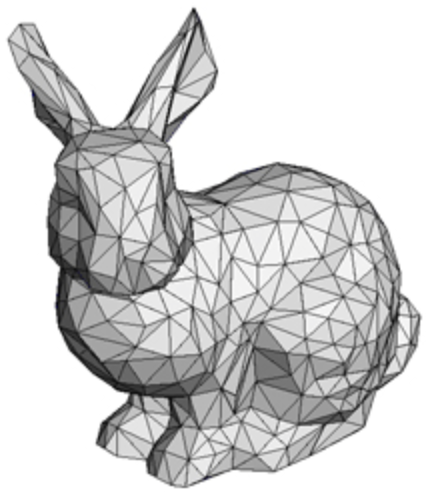
\includegraphics[width=5cm]{kanin}
    \caption{Eksempel hvor trekanter bruges til at repræsentere et objekt: http://www.cs.rpi.edu}
\end{figure}

For at rendere et billede af en 3D-model bestående af trekanter, er man nødt til at have en model for det kamera, som billedet renderes ud fra. Hvordan kameraet kan modelleres er beskrevet i næste afsnit.

\paragraph{Kamera}
Et kamera i konteksten af at rendere en 3D-model, er typisk en beskrivelse af position, orientation og synsfelt. Andre informationer kan tilknyttes som beskriver opløsning af det renderede billede, samt perspektivet af det resulterende billede. Orientationen fastsættes ved hjælp af et sæt vektorer som beskriver hvilken retning der er f.eks.\ højre og op for kameraret.

\begin{figure}[H]
  \centering
  \tdplotsetmaincoords{60}{130}
\begin{tikzpicture}[tdplot_main_coords]
\path[fill=gray!20, draw=gray!40] (-3,-4,-3) -- (-3,-4,3) -- (3,-4,3) -- (3,-4,-3) -- (-3,-4,-3);
\draw (0,0,0) -- (0,-4,0);
\draw[blue!50, thick, -{Stealth[width=2mm, length=2mm]}] (0,0,0) -- (0,-1,0);
\draw[blue!50, thick, -{Stealth[width=2mm, length=3mm]}] (0,-4,0) -- (-1,-4,0);
\draw[blue!50, thick, -{Stealth[width=2mm, length=2mm]}] (0,-4,0) -- (0,-4,1);
\draw[blue!50, thick, -{Stealth[width=2mm, length=2mm]}] (0,0,0) -- (-0.41,-0.8,0.41);
\draw[black, thick, dashed] (-0.41,-0.8,0.41) -- (-2,-4,2);
\draw[black, dashed, thick] (-0,-4,1) -- (-0,-4,2);
\draw[black, dashed, thick] (-0,-4,2) -- (-2,-4,2);
\draw[black, dashed, thick] (-1,-4,0) -- (-2,-4,0);
\draw[black, dashed, thick] (-2,-4,0) -- (-2,-4,2);
\draw plot [mark=*, mark size=2] coordinates{(0,0,0) }; 
\draw plot [mark=*, mark size=2] coordinates{(-2,-4,2) }; 
\node [below] at (0,0,0) {$C$};
\node [below] at (0,-1,-0.1) {$\vv{f}$};
\node [above right] at (0,-2.5,0) {$d$};
\node [above right] at (-2,-4,2) {$B$};
\node [left] at (-2,-4,1) {$y$};
\node [above] at (-1,-4,2) {$x$};
\node [above] at (-1,-4,0) {$\vv{r}$};
\node [right] at (-0.41,-0.8,0.41) {$\vv{s}$};
\node [left] at (0,-4,1) {$\vv{u}$};
\draw[blue!50, thick, |-|] (3.1,-4,3.2) -- (-2.9,-4,3.2);
\draw[blue!50, thick, |-|] (3.2,-4,3.1) -- (3.2,-4,-2.9);
\node [above] at (0,-4,3.2) {$w$};
\node [left]  at (3.2,-4,0) {$h$};
\end{tikzpicture}
  \caption{Visualisering af et punkt på billedplanet som en kombination af tre vektorer $\protect\vv{r}$, $\protect\vv{u}$ og $\protect\vv{f}$, der repræsenterer hhv. højre, op og frem retninger for kameraet.}
  \label{fig:kamera_billede}
\end{figure}

Et punkt $B$ på billedplanet (Se figur \ref{fig:kamera_billede}) kan repræsentere en pixel og kan beskrives som en lineær kombination af en op og en højre orientationsvektor samt en vektor der beskriver afstanden til billedplanet relativt til kammeraet. På figuren er denne vektor $\vv{f}$ skaleret med en faktor $d$.

En stråles retning gennem et pixel koordinat $B$ relativt til kameraets udgangspunkt $C$ kan altså beskrives på følgende måde:
\begin{align}
  \vv{B} &= C + \vv{f} \cdot d + \vv{u} \cdot (y-\frac{h}{2}) + \vv{r} \cdot (x-\frac{w}{2}) \\
  \vv{s} &= \frac{\vv{B}-\vv{C}}{||\vv{B}-\vv{C}||}
\end{align}

Hvor $(x,y)$ er en et koordinat mellem $(0,0)$ og $(w,h)$.

Afstanden $d$ samt størrelsen af billedplanet bestemmer forvrængningen af perspektiv projektionen.

\paragraph{Perspektiv projektion}
\label{sec:perspektiv_projektion}
For at udlede en model for billeddannelsen, tages der udgangspunkt i en perspektiv projektion. Perspektiv projektion er en måde at danne et billede af 3D-objekter ved at projektere objekterne hen på et plan mod et kameras position \cite{perspektive_projection}. Princippet bag perspektiv projektion er vist på figur \ref{fig:perspektiv_projektion}.

\begin{figure}[H]
  \centering
  \tdplotsetmaincoords{60}{130}
\begin{tikzpicture}[tdplot_main_coords]
\path[fill=blue!50, draw=gray!20] (2,-8,2) -- (-2,-8,2) -- (0,-8,0) -- (2,-8,2);
\draw (1,-4,1) -- (2,-8,2);
\draw (-1,-4,1) -- (-2,-8,2);
\draw (0,-4,0) -- (0,-8,0);
\path[fill=gray!20, draw=gray!40] (-2,-4,-2) -- (-2,-4,2) -- (2,-4,2) -- (2,-4,-2) -- (-2,-4,-2);
\path[fill=blue!50, draw=gray!20] (1,-4,1) -- (-1,-4,1) -- (0,-4,0) -- (1,-4,1);
\draw (0,0,0) -- (1,-4,1);
\draw (0,0,0) -- (-1,-4,1);
\draw (0,0,0) -- (0,-4,0);

\draw plot [mark=*, mark size=2] coordinates{(2,-8,2) } ; 
\draw plot [mark=*, mark size=2] coordinates{(-2,-8,2) } ; 
\draw plot [mark=*, mark size=2] coordinates{(0,-8,0) } ; 
\draw plot [mark=*, mark size=2] coordinates{(1,-4,1) }; 
\draw plot [mark=*, mark size=2] coordinates{(-1,-4,1) }; 
\draw plot [mark=*, mark size=2] coordinates{(0,-4,0) }; 
\draw plot [mark=*, mark size=2] coordinates{(0,0,0) }; 
\node [above left] at (2,-8,2) {$P$};
\node [above left] at (1,-4,1) {$B$};
\node [above right] at (0,0,0) {$C$};
\end{tikzpicture}
  \caption{Viser princippet bag perspektiv projektion af et punkt på et billedplan.}
  \label{fig:perspektiv_projektion}
\end{figure}

Som vist på figur \ref{fig:perspektiv_projektion} kan et punkt $P\in \mathbb{R}^3$ projekteres ned på billedplanen $\alpha$ ved at finde skæringspunktet $B$ mellem billedplanen $\alpha$ og en lysstråle $L$, som går fra punktet $P$ mod kameraets position $C$. Gør man nu dette for alle punkter på et objekt i rummet, og tegner skæringspunkterne på billedplanen, dannes et billede af objektet, ved at oversætte punktet på billedplanen, til (x,y)-pixelkoordinater, på det resulterende billede, med udtrykket beskrevet under afsnittet om kameraet.

Udfordringen er så at afgøre hvilken farve punkterne på billedplanen skal have, da dette afhænger af objektets egenskaber, samt hvilket udefrakommende lys der rammer objektet. 

For at løse denne udfordring, benytter vi i dette projekt raytracing, der som beskrevet under afsnit \ref{sec:computergrafik}, bygger på at simulere lysstrålers interaktion med forskellige objekter i rummet. Hvordan dette fungere er beskrevet i næste afsnit, hvor der er beskrevet en model for backwards raytracing.

\paragraph{Backwards raytracing}
I modsætning til en perspektiv projektion af et punkt på et plan, er backwards raytracing, hvor man i stedet for punktet i rummet, tager udgangspunkt i de lysstråler der danner billedet. Ved backwards raytracing følger man lysstrålerne baglæns og ser på, hvor stor en lysintensitet, den pågældende lysstråle har efter den har interageret med objekterne i rummet. Ud fra dette farves det tilhørende punkt på billedet, og på den måde kan man rendere et helt billede. På figur \ref{fig:raytracing_skitse} er det vist hvordan man kan konstruere en lysstråle ud fra et bestemt punkt på billedplanen, hvor lysstrålen er beskrevet ved en retningsvektor og et startpunkt.

\begin{figure}[H]
  \centering
  \tdplotsetmaincoords{60}{130}
  \begin{tikzpicture}[tdplot_main_coords]
  \path[fill=blue!50, draw=gray!20] (2,-8,2) -- (-2,-8,2) -- (0,-8,0) -- (2,-8,2);
\draw (0,0,0) -- (0,-8,1);
\path[fill=gray!20, draw=gray!40] (-2,-4,-2) -- (-2,-4,2) -- (2,-4,2) -- (2,-4,-2) -- (-2,-4,-2);
\draw plot [mark=*, mark size=2] coordinates{(0,-4,0.5) }; 
\draw plot [mark=*, mark size=2] coordinates{(0,0,0) }; 
\node [above right] at (0,-4,0.5) {$B$};
\node [above right] at (0,0,0) {$C$};
\draw [blue!50, thick, -{Stealth[width=3mm, length=3mm]}] (0,0,0) -- (0,-4,0.5);
\node [above right] at (0,-2,0.25) {$\vv{r}$};
\end{tikzpicture}
  \caption{Viser hvordan en der kan opstilles retningsvektor mellem kameraets position $C$ og punktet $P$ på billedplanen, som sammen med startpunktet $C$ beskriver lysstrålen fra trekanten i omvendt retning.}
  \label{fig:raytracing_skitse}
\end{figure}

Retningsvektoren $\vv{r}$ for lysstrålen kan heraf beskrives som følgende.

$$ \vv{r} = \vv{B} - \vv{C} $$

Hvor $\vv{B}$ og $\vv{C}$ er stedvektorer for hhv. punktet på billedplanen $B$ og kameraets position $C$.

Lysstrålen kan på den måde beskrives ved følgende vektorfunktion.

$$ \vv{l}(t) = \vv{r} t + \vv{C}$$

Hvor $t$ er en skalar i $\mathbb{R}$.

For at finde ud af hvilken farve punktet på billedplanen $B$ skal have, ser man hvordan lysstrålen rammer de forskellige objekter der skal renderes.

Der findes flere forskellige modeller for hvordan lysintensiteten for en lysstråle beregnes. En simpel model, er Phong-modellen, som opdeler lys i forskellige kategorier: ambient, diffuse og specular.

\paragraph{Phong-modellen}
Phong-modellen er en såkaldt \textit{shading} funktion, som beskriver lyset fra punkter på et objekt på baggrund af lyskilden, objektet og kameraets synsvinkel\cite{phong_paper}. Der findes flere forskellige variationer af phong-modellen. Da vi som vist i afsnit \ref{sec:temptilrgb} kan arbejde med farvetemperaturer via rgb-værdier, så har vi valgt en variation af phong-modellen, som beskriver lys via rgb-værdier. 

Ud fra modellen\cite{stanford_phong}, kan der skrives følgende overordnede \textit{shading} funktion.
\begin{equation} \label{eq:phong}
  \rho = \rho_a + \sum\limits_{lights} (\rho_d + \rho_s)
\end{equation}
Hvor $\rho_a$, $\rho_l$ og $\rho_s$ er hhv. \textit{ambient}, \textit{diffuse} og \textit{specular} lys der er beskrevet kort herunder.

\subparagraph{\textit{Ambient} lys} repræsenterer det lys, som reflekteres rundt i rummet og rammer objekter ligeligt fra alle sider\cite{stanford_phong}. Formlen til at beregne dette er følgende\cite{stanford_phong}.
\begin{align}
\label{eq:ambient_formel}
	\rho_a &= m_a C A
\end{align}
Hvor $m_a$ er den ambiente konstant, $C$ er overfladens farve som rgb-værdi og $A$ er den ambiente lysintensitet.

\subparagraph{\textit{Diffuse} lys} er det lys, som reflekteres ifølge \textit{Lambert's Cosinuslov}. Ud fra loven kan følgende model anvendes til at udregne \textit{diffuse} lys\cite{stanford_phong}.
\begin{align}
	\rho_l &= m_l C I max(\vv{I}\bullet\vv{n}, 0)
\end{align}
Hvor $m_l$ er den Lambertianske konstant, $I$ er det lyskildens lysintensitet, $\vv{I}$ og $\vv{n}$, er normaliserede vektorer, hhv. vektor fra overfladepunktet mod lyskilden og normalvektoren til overfladepunktet.

\subparagraph{\textit{Specular} lys} er det lys der spejles i objektets overflade, givet ved nedenstående formel\cite{stanford_phong}.
\begin{align}
	\rho_s &= m_s S I max(\vv{r}\bullet\vv{u},0)^{m_{sp}} \\
	S &= m_{sm} C + (1 - m_{sm})(1,1,1)
\end{align}
Hvor $m_s$ er den specular konstant, $S$ er en lineær interpolation mellem objektets farve og hvid, afhængig af objektets \textit{metalness} $m_{sm}$. $\vv{u}$ og $\vv{r}$ er normaliserede vektorer, for hhv. vektor fra overfladepunktet mod kameraet og retningsvektor for det reflekterede lys beregnet som følgende.
\begin{align}
	\vv{r} &= -\vv{I} + 2 (\vv{I} \bullet \vv{n}) \vv{n}
\end{align}

De anvendte vektorer til phong \textit{shading} funktionen er vist på figuren herunder.
\begin{figure}[H]
  \label{fig:phong_skitse}
  \centering
  \tdplotsetmaincoords{60}{130}
  \begin{tikzpicture}[tdplot_main_coords]
  \draw plot [mark=*, mark size=2] coordinates{(0,-4,2) }; 
\node [above left] at (0,-4,2) {$C$};
  \draw (0,-4,2) -- (0,-3,1.5);
  \path[fill=gray!20, draw=gray!40] (-1,-3,1) -- (-1,-3,3) -- (1,-3,3) -- (1,-3,1);

  \path[fill=gray!20, draw=gray!40] (1,-2,0) -- (-1,0,0) -- (1,2,0);
    \draw (0,-3,1.5) -- (0,0,0);
    \draw [blue!50, thick, -{Stealth[width=3mm, length=3mm]}] (0,0,0) -- (0,0,2.24);
    \node [above] at (0,0,2.24) {$\vv{n}$};
    \draw [blue!50, thick, -{Stealth[width=3mm, length=3mm]}] (0,0,0) -- (0,-2,1);
    \node [below left] at (0,-2,1) {$\vv{u}$};
    \draw [blue!50, thick, -{Stealth[width=3mm, length=3mm]}] (0,0,0) -- (0,-1,2);
    \node [above left] at (0,-1,2) {$\vv{r}$};
    \draw (0,0,0) -- (0,2,4);
    \draw plot [mark=*, mark size=2] coordinates{(0,2,4) }; 
    \node [above right] at (0,2,4) {$L$};
    \draw [blue!50, thick, -{Stealth[width=3mm, length=3mm]}] (0,0,0) -- (0,1,2);
    \node [right] at (0,1,2) {$\vv{I}$};
 \draw (0,0.3, 1.1) -- (0,0.35, 1.3);
  \draw (0,0.35, 1.1) -- (0,0.4, 1.3);
  
 \draw (0,-0.2, 0.9) -- (0,-0.25, 1.1);
  \draw (0,-0.15, 0.95) -- (0,-0.2, 1.15);

  \draw (0,-1,2) coordinate (a)
  (0,0,0) coordinate (b)
  (0,0,2.24) coordinate (c)
  pic[draw=black,|-|,angle eccentricity=1.2,angle radius=1cm] {angle=c--b--a};
  \draw (0,0,2.24) coordinate (a)
  (0,0,0) coordinate (b)
  (0,1,2) coordinate (c)
  pic[draw=black,|-|,angle eccentricity=1.2,angle radius=1cm] {angle=c--b--a};
\draw plot [mark=*, mark size=2] coordinates{(0,0,0) }; 
    \node [below right] at (0,2,4) {$P$};
\end{tikzpicture}
  \caption{Viser vektorer der anvendes i phong-modellen. $\protect\vv{u}$ er vektor mod kameraet med position $C$, $\protect\vv{n}$ er normalvektoren til objektet i punktet $P$, $\protect\vv{I}$ er vektor mod lyskildens position $L$ og $\protect\vv{r}$ er vektor for det reflekterede lys.}
\end{figure}

\subsubsection{Skæring mellem linje og trekant i rummet}
\label{sec:triangle_intersection}
For at finde om der er en skæring mellem en stråle og en trekant, kan man følge tre trin:
\begin{enumerate}
  \item Find skæringen med trekantens plan og påvis at punktet er foran strålens udgangspunkt
  \item Påvis at punktet i trekantens plan, ligger indenfor trekanten
  \item Påvis at strålens linje ikke er parallel med trekantens plan
\end{enumerate}

En stråle er paralel med et plan hvis strålens retning er 90 grader relativt til planets normalvektor, dette er sandt hvis ligning \ref{eq:parralel} er opfyldt.

\begin{equation}
  \label{eq:parralel}
  \vv{r} \bullet \vv{n} = 0
\end{equation}

Planets normalvektor findes ved at krydse to vektore fra en af trekantens hjørner til de to andre (se ligning \ref{eq:triangle_normal}).

\begin{equation}
  \label{eq:triangle_normal}
  \vv{n} = (B - A) \times (C - A)
\end{equation}

\begin{figure}[H]
  \centering
  \tdplotsetmaincoords{60}{130}
  \begin{tikzpicture}[tdplot_main_coords]
    % dashed line through plane
    \draw [black, thick] (0,0,0) -- (4,-8,4);
    % triangle and plane
    \path[fill=gray!10, draw=gray!20] (0,-4,0) -- (4,-4,0) -- (4,-4,4) -- (0,-4,4) -- (0,-4,0);
    \path[fill=gray!30, draw=gray!60] (1,-4,2) -- (2,-4,3) -- (3,-4,1) -- (1,-4,2);
    % triangle
    \draw [blue!50, thick, -{Stealth[width=3mm, length=3mm]}] (2,-4,3) -- (3,-4,1);
    \draw [blue!50, thick, -{Stealth[width=3mm, length=3mm]}] (2,-4,3) -- (1,-4,2);
    \draw [blue!50, thick, -{Stealth[width=3mm, length=3mm]}] (2,-4,3) -- (2,-2,3);
    % \draw [black,   thick, -{Stealth[width=2mm, length=2mm]}] (2,-4,3) -- (2,-4,2);
    \node [above] at (2,-3,3) {$\vv{n}$};
    \node [above] at (2,-4,3) {$A$};
    \draw plot [mark=*, mark size=1] coordinates{(2,-4,3) }; 
    \node [left] at (3,-4,1) {$B$};
    \draw plot [mark=*, mark size=1] coordinates{(3,-4,1) }; 
    \node [below] at (1,-4,2) {$C$};
    \draw plot [mark=*, mark size=1] coordinates{(1,-4,2) };
    
    % ray
    \node [above right] at (0,0,0) {$P_0$};
    \draw plot [mark=*, mark size=1] coordinates{(0,0,0) };
    \node [above right] at (0.25,-0.5,0.25) {$\vv{r}$};
    \draw [black, thick] (0,0,0) -- (2,-4,2);
    \draw [blue!50, thick, |-|] (0.1,0,-0.1) -- (2.1,-4,1.9);
    \node [below left] at (1,-2,1) {$t_A$};
    \node [black, above left] at (2.5,-4,2) {$P(t_A)$};
    \draw [black, thick, -{Stealth[width=3mm, length=3mm]}] (0,0,0) -- (0.5,-1,0.5);
    \draw plot [mark=*, mark size=1] coordinates{(2,-4,2) };
  \end{tikzpicture}
  \caption{Viser princippet bag perspektiv projektion af et punkt på et billedplan.}
  \label{fig:perspektiv_projektion}
\end{figure}

Hvis strålen ikke er parralel med planet kan vi nu finde et punkt i planet som strålen skære. Alle vektore i planet er ortogonale på normal vektoren, dermed kan vi opstille ligning \ref{eq:vektor_in_plane} til at beskrive betingelsen for et punkt strålen som også ligger i planet. Ved at substituere linjens ligning (ligning \ref{eq:point_on_ray}) ind og isolere $t_A$ kan vi så bruge til at finde punktet på strålens linje og er $t_A > 0$ så er punktet også foran strålens udgangspunkt $P_0$

\begin{align}
  \label{eq:point_on_ray}
  P(t) &= \vv{r} \cdotp t + \vv{P_0} \\
  \label{eq:vektor_in_plane}
  ( P(t_A) - A ) \bullet \vv{n} &= 0 \\
  \label{eq:test3}
  (\vv{r} \cdotp t_A + \vv{P_0} - A) \bullet \vv{n} &= 0 \\
  \label{eq:test4}
  t_A \cdotp \vv{r} \bullet \vv{n} + (\vv{P_0} - A) \bullet \vv{n} &= 0 \\
  \label{eq:test5}
  t_A &= -\frac{(\vv{A} - \vv{P_0})\bullet \vv{n}}{\vv{r} \bullet \vv{n}}
\end{align}


[FIND IF POINT IS INSIDE TRIANGLE]()

\begin{figure}[H]
  \centering
  \tdplotsetmaincoords{60}{130}
  \begin{tikzpicture}[tdplot_main_coords,thick,scale=2, every node/.style={transform shape}]
    \coordinate (Pt) at (2,-4,2);
    \coordinate (A) at (2,-4,3);
    \coordinate (B) at (3,-4,1);
    \coordinate (C) at (1,-4,2);
    % dashed line through plane
    % triangle and plane
    \path[fill=gray!10, draw=gray!20] (0.8,-4,0.8) -- (3.2,-4,0.8) -- (3.2,-4,3.2) -- (0.8,-4,3.2) -- (0.8,-4,0.8);
    \path[fill=gray!30, draw=gray!60] (A) -- (B) -- (C) -- (A);
    % triangle
    \draw [blue!50, thick, -{Stealth[width=3mm, length=3mm]}] (A) -- (B);
    \draw [blue!50, thick, -{Stealth[width=2mm, length=2mm]}] (A) -- (Pt);
    \draw [blue!50, thick, -{Stealth[width=3mm, length=3mm]}] (B) -- (C);
    \draw [blue!50, thick, -{Stealth[width=2mm, length=2mm]}] (B) -- (Pt);
    \draw [blue!50, thick, -{Stealth[width=3mm, length=3mm]}] (C) -- (A);
    \draw [blue!50, thick, -{Stealth[width=2mm, length=2mm]}] (C) -- (Pt);
    \node [above] at (2,-3,3) {$\vv{n}$};
    \node [above] at (2,-4,3) {$A$};
    \draw plot [mark=*, mark size=1] coordinates{(2,-4,3) }; 
    \node [left] at (3,-4,1) {$B$};
    \draw plot [mark=*, mark size=1] coordinates{(3,-4,1) }; 
    \node [below] at (1,-4,2) {$C$};
    \draw plot [mark=*, mark size=1] coordinates{(1,-4,2) };
    
    % ray
    \node [black, above left] at (2.5,-4,2) {$P(t_A)$};
    \draw plot [mark=*, mark size=1] coordinates{(2,-4,2) };
  \end{tikzpicture}
  \caption{Viser princippet bag perspektiv projektion af et punkt på et billedplan.}
  \label{fig:perspektiv_projektion}
\end{figure}


\subsubsection{Kd-træer}
\label{sec:kdtree}

Kd-træer er binære træer, hvilket betyder at hver node maksimalt har to under-noder. K'et i kd-træ er antallet af dimensioner, men i stedet for 3D træ, siger man et 3-dimensionelt kd-træ. Kd-træer bruges til at minimere antallet af søgninger, som et givent program skal gennemføre. 

Et kd-træ opbygges ved at have en mængde af værdier, som er usorterede. Disse værdier kan inddeles i et træ, ved at finde et taktisk splittepunkt, som er roden. Herefter går to noder ud fra roden, den venstre har den nedre halvdel af værdierne og den højre har den øvre halvdel. Herefter splittes disse to noder hver for sig igen, og sådan fortsætter træet indtil fastsatte krav nås, hvorefter man så kalder den sidste række af noder for bladene. 

En simpel forklaring af et to-dimensionelt kd-træ kan være et program til at finde tallet 100 i en tilfældig mængde fra 1-1000. Roden deles på et bestemt punkt, hvilket i dette tilfælde er midtpå ved 500, og derfor vil den venstre under-node til 'rod-noden' indeholde værdier, der er lig med eller under 500 og det højre barn til indeholde værdier, der er højere end eller lig med 500. Sådan fortsætter programmet med at halvere alle muligheder efter hvert niveau indtil den ønskede værdi er fundet. Denne metode kræver i teorien færre sammenligninger og bør dermed være hurtigerer for store datasæt end hvis man bad et program om at finde et givent tal mellem 1 og 1000, da den, i værste tilfælde, skulle tjekke 999 tal igennem, før den fandt det ønskede nummer.

\begin{figure}[H]
  \centering
  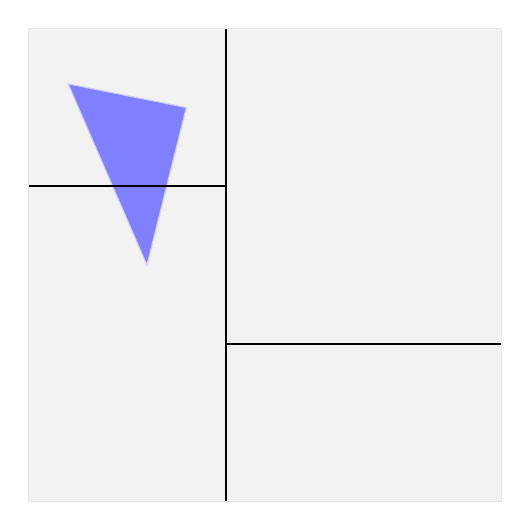
\begin{tikzpicture}
    \path[fill=gray!10, draw=gray!20] (3,3) -- (3,-3) -- (-3,-3) -- (-3,3) -- (3,3);
    
    \path[fill=blue!50, draw=blue!20] (-1,2) -- (-2.5,2.3) -- (-1.5,0) -- (-1,2);
    
    \draw [black, thick] (-0.5, -3) -- (-0.5, 3);
    \draw [black, thick] (-0.5, -1) -- ( 3,  -1);
    \draw [black, thick] (-0.5,  1) -- (-3,   1);
    % triangle
    % \draw [blue!50, thick, -{Stealth[width=3mm, length=3mm]}] (2,-4,3) -- (3,-4,1);
    % \draw [blue!50, thick, -{Stealth[width=3mm, length=3mm]}] (2,-4,3) -- (1,-4,2);
    % \draw [blue!50, thick, -{Stealth[width=3mm, length=3mm]}] (2,-4,3) -- (2,-2,3);
    % \draw [black,   thick, -{Stealth[width=2mm, length=2mm]}] (2,-4,3) -- (2,-4,2);
    % \node [above] at (2,-3,3) {$\vv{n}$};
    % \node [above] at (2,-4,3) {$A$};
    % \draw plot [mark=*, mark size=1] coordinates{(2,-4,3) }; 
    % \node [left] at (3,-4,1) {$B$};
    % \draw plot [mark=*, mark size=1] coordinates{(3,-4,1) }; 
    % \node [below] at (1,-4,2) {$C$};
    % \draw plot [mark=*, mark size=1] coordinates{(1,-4,2) };
    
    % ray
    % \node [above right] at (0,0,0) {$P_0$};
    % \draw plot [mark=*, mark size=1] coordinates{(0,0,0) };
    % \node [above right] at (0.25,-0.5,0.25) {$\vv{r}$};
    % \draw [black, thick] (0,0,0) -- (2,-4,2);
    % \draw [blue!50, thick, |-|] (0.1,0,-0.1) -- (2.1,-4,1.9);
    % \node [below left] at (1,-2,1) {$t_A$};
    % \node [black, above left] at (2.5,-4,2) {$P(t_A)$};
    % \draw [black, thick, -{Stealth[width=3mm, length=3mm]}] (0,0,0) -- (0.5,-1,0.5);
    % \draw plot [mark=*, mark size=1] coordinates{(2,-4,2) };
  \end{tikzpicture}
  \caption{KD-træ}
  \label{fig:kd-tree}
\end{figure}
---
% \begin{figure}[H]
%   \centering
%   \begin{tikzpicture}[
%     level 1/.style={sibling distance=40mm},
%     level 3/.style={sibling distance=20mm},
%     level 4/.style={sibling distance=10mm},
%     every node/.style={draw,circle},
%     arrow/.style={edge from parent/.style={draw,-latex}}
%   ]
%   \node {A}
%     child { node{B}
%       child { node{D}
%         child {node{H}}
%         child {node{I}}
%       }
%       child { node{E}
%         child {node{J}}
%         child {node{K}}
%       }
%     }
%     child { node{C}
%       child { node{F}
%         child {node{L}}
%         child {node{M}}
%       }
%       child { node{G}
%         child {node{N}}
%         child {node{O}}
%       }
%     }
%   ;
%   \end{tikzpicture}
%   \caption{KD-træ}
%   \label{fig:kd-tree}
% \end{figure}

\subsubsection*{Opsummering}

Ud fra teoridiskussionen kan der nu kortfattets hvordan teorierne bidrager til programudviklingen. 

Rotationsmatricer giver den viden som skal til for at roterer vektorer i rummet med en vilkårlig vinkel. Dette er relevant når man skal flytte kameraets position, som hører til programkravet om at lampens belysning skal kunne visualiseres fra flere forskellige vinkler.

Teorien om konvertering fra farvetemperatur til RGB giver os den algoritme som skal til for, at lave en farvetemperatur i kelvin om til en RGB-værdi. Dette er relevant i forhold til programkravet om at kunne ændre pærens farvetemperatur. 

Teorien fra 3D-model til billede omhandler matematiske modeller og beskrivelser af relevante teknologier og algoritmer. Teorien i dette er relevant for, at forstå nogle af grundprincipperne i en raytracer heriblandt backwards raytracing og Phong-modellen.

Teorien om ray-triangle intersection omhandler en matematisk model over, hvordan man finder skæringen mellem en ray og en trekant i planen. Dette knytter sig til teorien om en 3D-model, da alle objekter består af trekanter. 

Som afslutning på teoridiskussionen opstilles følgende nye krav til programudviklingen i forhold til kravene i afsnit \ref{sec:krav}:
\begin{enumerate}
    \item Programmet skal kunne modtage følgende input fra brugeren: 3D-fil af lampen og dens kontekst, billedets opløsning, pærens farvetemperatur og hvilken synsvinkel man ønsker at se billedet fra (kameraets position).
    \item Programmet skal ved brug af raytracing kunne fremstille et billede af lampen og dens belysning på baggrund af brugerinputtet. Derudover skal raytracerens renderingstid optimeres ved brug af KD-træer.
    \item Programmet skal kunne gemme det renderede billede.
\end{enumerate}

\subsubsection{Fra 3D-model til billede}
I dette afsnit er det vist, hvordan der kan udledes en model, der beskriver en billeddannelsen af objekter i rummet, også kaldt rendering. Dette er essentielt da billeddannelsen danner grundlag for, hvordan 3D-modellen for en lampe omdannes til et billede, der kan vises for kunderne på e-butikken. Til sidst i afsnittet udledes en model for, hvordan belysningen fra en lampe kan simuleres og visualiseres vha. raytracing. 

\paragraph{Perspektiv projektion}
For at udlede en model for billeddannelsen, tages der udgangspunkt i en perspektiv projektion. Perspektiv projektion er en måde at danne et billede af 3D-objekter ved at projektere objekterne hen på et plan mod et kameraes position\cite{fig:perspective_projection}. Princippet bag perspektiv projektion er vist på figur \ref{fig:perspektiv_projektion}.

\begin{figure}[H]
  \label{fig:perspektiv_projektion}
  \centering
  \tdplotsetmaincoords{60}{130}
\begin{tikzpicture}[tdplot_main_coords]
\draw (0,0,0) -> (2,-8,2);
\path[fill=gray!30, draw=gray] (-2,-4,-2) -- (-2,-4,2) -- (2,-4,2) -- (2,-4,-2) -- (-2,-4,-2);
\draw (0,0,0) -- (1,-4,1);
\foreach \p in {(2,-8,2),(1,-4,1),(0,0,0)}{
	\draw plot [mark=*, mark size=2] coordinates{\p } ; 
	\node [above right] at \p {P};
}
\draw plot [mark=*, mark size=2] coordinates{(2,-8,2) } ; 
\draw plot [mark=*, mark size=2] coordinates{(1,-4,1) }; 
\draw plot [mark=*, mark size=2] coordinates{(0,0,0) }; 
\node [above right] at (2,-8,2) {P};
\node [above right] at (1,-4,1) {B};
\node [above right] at (0,0,0) {C};
\end{tikzpicture}
  \caption{Viser princippet bag perspektiv projektion af et punkt på et billedplan.}
\end{figure}



Som vist på figur \ref{fig:perspektiv_projektion} kan et punkt $P\in \mathbb{R}^3$ projekteres ned på billedplanen $\alpha$ ved at finde skæringspunktet $B$ mellem billedplanen $\alpha$ og en lysstråle $L$, som går fra punktet $P$ mod kameraets position $C$. Gør man nu dette for alle punkter på et objekt i rummet, og tegner skæringspunkterne på billedplanen, dannes et billede af objektet. Udfordringen er så at afgøre hvilken farve punkterne på billedplanen skal have, da dette afhænger af objektets egenskaber, samt hvilket udefrakommende lys der rammer objektet. 

For at løse denne udfordring, benytter vi i dette projekt raytracing, der som beskrevet under afsnit \ref{sec:computergrafik}, bygger på at simulere lysstrålers interaktion med forskellige objekter i rummet. Hvordan dette fungere er beskrevet i næste afsnit, hvor der er beskrevet en model for backwards raytracing.

\paragraph{Raytracing}
I modsætning til en perspektiv projektion af et punkt på et plan, er raytracing, hvor man i stedet for punktet i rummet, tager udgangspunkt i de lysstråler der danner billedet. Ved backwards raytracing følger man lysstrålerne baglæns og ser på, hvor stor en lysintensitet, den pågældende lysstråle har efter den har interageret med objekterne i rummet. Ud fra dette farves det tilhørende punkt på billedet, og på den måde kan man rendere et helt billede. På figur \ref{fig:raytracing_skitse} er det vist hvordan man kan konstruere en lysstråle ud fra et bestemt punkt på billedplanen, hvor lysstrålen er beskrevet ved en retningsvektor og et startpunkt.

\begin{figure}[H]
  \label{fig:raytracing_skitse}
  \centering
  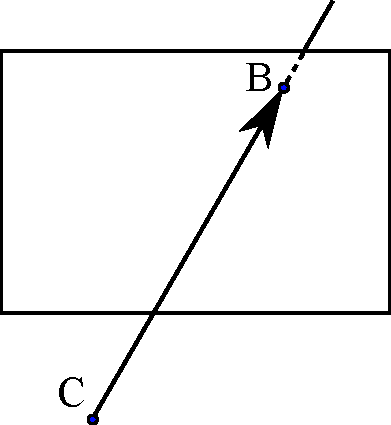
\includegraphics[width=5cm]{drawing}
  \caption{Viser hvordan en der kan opstilles retningsvektor mellem kameraets position $C$ og punktet $P$ på billedplanen, som sammen med startpunktet $C$ beskriver lysstrålen i omvendt retning.}
\end{figure}

Der findes flere forskellige modeller for hvordan lysintensiteten for en lysstråle beregnes. En simpel model, er Phong-modellen, som opdeler lys i forskellige kategorier: ambient, diffuse og specular.


\subsection{Udvikling}
Formålet med dette afsnit er, at give en beskrivelse af programmets opbygning og struktur, samt ved brug af kodeeksempler og teori beskrevet i \ref{sec:teori}, at forklare hvordan funktionerne i programmet virker og hvad de gør. I afsnittet vil der være kodeeksempler på prototyperne til funktionerne og kodeeksempler på selve funktionen. Hele programmet kan findes online som elektronisk bilag.

\subsubsection{Datastrukturer}
[Indledning: Forklar at vi bruger datastrukturer for at abstrahere over data.]
\paragraph{Vektor}
En stor del af opgaven bygger på vektorer i rummet. Nedenstående kodeuddrag viser hvordan der er abstraheret over en vektor i programmet. 

\begin{lstlisting}[style=Cstyle, caption=Struct til vektor]
typedef struct _vector {
    double x, y, z;
} Vector;
\end{lstlisting}

På linje 2 i ovenstående kodeuddrag er det vist hvordan en 3D vektors koordinarter er beskrevet med typen double. 

\paragraph{Stråle}
For at benytte sig af ray-tracingmetoden er det naturligvis nødvendigt at have en ray (stråle) som man kan trace (følge). 

\begin{lstlisting}[style=Cstyle, caption=Struct til ray]
typedef struct _ray {
  Vector initial_point, direction;
} Ray;
\end{lstlisting}

På linje to i ovenstående kodeuddrag kan det ses at en ray består af et startpunkt (initial_point) og en retning, begge af disse er af typen Vector, som tidligere er beskrevet til at have et x-, y- og z-koordinat.

\paragraph{Trekant}
Enhver figur i programmet består af mange sammensatte trekanter. I de fleste tilfælde er det så mange trekanter, at det ikke umiddelbart er synligt for det blotte øje. Et hjørne i en trekant udspændes af flere og kaldes en vertex.
    
\begin{lstlisting}[style=Cstyle, caption=Struct til vertex]
typedef struct _verticie {
  Vector position;
  Vector normal;
} Vertex;
\end{lstlisting}

På linje to og tre i ovenstående kodeuddrag kan det ses at en vertex består af et stedvektor, som er kaldet position, og en normalvektor.
    
Som nævnt for ovenstående struct for en vertex, er alle objekter i programmet bestående af trekanter. Nedenstående kodeuddrag viser hvordan trekanter er implementeret i programmet.
    
\begin{lstlisting}[style=Cstyle, caption=Struct til triangle]
typedef struct _triangle {
  Vertex *verticies[3];
  Vector edges[3];
} Triangle;
\end{lstlisting}

Denne struct viser, kort sagt, at en trekant består af tre hjørner, altså tre verticies, af typen Vertex, samt tre edges, der er stedvektorer til de tre verticies.

\paragraph{Point\_lights}

En raytracers formål er at følge lysstrålerne, som udskydes fra et bestemt punkt, som i vores tilfælde er fra en pære. 

\begin{lstlisting}[style=Cstyle, caption=Struct til light]
typedef struct _pointlight {
  Vector position;
  Pixel color;
  double intensity;
  double radius;
  int sampling_rate;
} PointLight;
\end{lstlisting}

På linje to i ovenstående kodeuddrag kan det ses, at et lys har en given position, som bestemmes af ét 3D-koordinat. Dette lys har en farve, bestående af en RGB-værdi. Derudover har lyset også en intensitet og radius af typen double, samt sampling_rate af typen int.

\paragraph{Materiale}
I virkeligheden har vi mange forskellige materialer der både syner og føles anderledes end andre. En helt ny bil skinner når man lyser på den, mens en murstensvæg er helt mat. For at illustrere det i raytracing har vi brugt nogen værdier der ofte bruges i forbindelse med 3D-rendering og især raytracing. Vi har valgt at bruge Phong-modellen da den er relativ simpel og giver et godt resultat.

\begin{lstlisting}[style=Cstyle, caption=Struct til Material]
typedef struct _material {
  double ambient_coefficient;
  double diffuse_coefficient;
  double specular_coefficient;
  int smoothness;
  double metalness; 
} Material;
\end{lstlisting}

Ambient_coefficient er værdien der fortæller hvor lyst objektet er selvom der ikke er direkte lys på den. Den bevirker at hvis objektet er i skygge så er det ikke helt sort.
Diffuse_coefficient er skygge-værdien der viser hvor stor indflydelse lys har på objektet. 
Specular_coefficient er værdien der viser hvor meget objektet spejler igen. Denne værdi er høj for en ny poleret bil, men næsten 0 hvis det er en murstensvæg. I vores program gør det at vi får en næsten hvid plet hvis vores lyskilde spejler igen.

\paragraph{AABB}
AABB står for axis aligned bounding boxes, og er en kasse hvis sidder er parallelle med akserne. En boks består af to vektorer som indeholder det laveste og største koordinatsæt for boksen. De to vektorer er en stedvektor til det hjørne på boksen som er tættest på og længst væk fra origo. Nedenstående kodeuddrag viser hvordan dette er gjort i programmet.

\begin{lstlisting}[style=Cstyle, caption=Struct til bounding boxes]
typedef struct _plane {
  Vector low, high;
\end{lstlisting}

De to punkter til boksen er angivet som stedvektorer af typen vector (linje 2).

\paragraph{Plan}
Et plan i rummet er beskrev ved et punkt og en normalvektor til planen. Hvordan dette er gjort i programmet er vist i nedenstående kodeuddrag. 

\begin{lstlisting}[style=Cstyle, caption=Struct til plan]
typedef struct _plane {
  Vector normal;
  Vector point;
\end{lstlisting}

Planens normalvektor er beskrevet med typen vector (linje to). Et punkt til planen er angivet som en stedvektor af typen vector (linje tre).

\paragraph{Skæring}
Det er nødvendigt at vide, hvis og hvor en lysstråle skærer et objekt, for at finde de data (farve, materiale, lokation m.m.) der er i det givne punkt ved skæringen.

\begin{lstlisting}[style=Cstyle, caption=Struct til intersection]
typedef struct _intersection {
  Vector normal;
  Material material;
  Pixel color;
  Triangle *triangle;
  Ray ray;
  double t;
} Intersection;
\end{lstlisting}

På ovenstående struct kan det ses, at hver intersection har en mængde data, som bruges senere til phong. Hver intersection har en 
normalvektor, et materiale, en farve beskrevet ved typen Pixel. Den har derudover en 'triangle' til at finde hvilken trekant i træet, som den skærer i, en 'ray', som beskriver lysstrålen, der skærer i det givne punkt samt en tid t af typen double, der beskriver afstanden fra initialpoint.

\paragraph{Billede}
Vi har en Image-struct for at simplificerer måden vi udskriver pixels på og forbedre læseligheden.

\begin{lstlisting}[style=Cstyle, caption=Struct til Image]
typedef struct _image {
  unsigned int width, height;
  Pixel **pixels;
} Image;
\end{lstlisting}

Vores Image-struct definerer 2 doubles der beskriver højden og bredden på vores billede i pixels.
Vi har også et 2-dimensionelt array med Pixels der beskriver vores billede.

\paragraph{Kamera}
Som vist på figur \ref{...} i afsnit \ref{...} er kameraet beskrevet som dens position og orientering i rummet samt en afstand, d, til kameraet. Derudover har kameraet en højde og en bredde som definerer billedets opløsning. Nedenstående kodeuddrag viser hvordan dette er gjort i programmet.

\begin{lstlisting}[style=Cstyle, caption=Struct til kamera]
typedef struct _camera {
  Vector up;
  Vector right;
  Vector forward;
  Vector position;
  unsigned int width, height;
  double distance;
} Camera;
\end{lstlisting}

Kameraets orientering kan beskrives som tre vektorer af typen vector (linje 2-4). Kameraets position kan angives som en stedvektor af typen vector (linje 5). Opløsningen er angivet som positive heltal af typen unsigned int (linje 6). Afstanden til kameraet er angivet som typen double (linje 7).

\paragraph{Scene}
Scenen er den virtuelle verden, som skal visualiseres. I programmet er scenen beskrevet på følgende måde. 

\begin{lstlisting}[style=Cstyle, caption=Struct til scene]
typedef struct _scene {
  Object **objects;
  unsigned int n_objects;
  PointLight **lights;
  unsigned int n_lights;
  Pixel ambient_intensity;
} Scene; 
\end{lstlisting}

En scene består af en række objekter (linje 2-3), en række lys (linje 4-5), samt den ambiente lys intensitet der bruges i Phong.

\paragraph{Objekt}
Objektet er det man kan se når billedet bliver renderet af raytraceren. I programmet er objektet beskrevet på følgende måde.

\begin{lstlisting}[style=Cstyle, caption=Structs til objektet]
typedef struct _object {
  Vertex *verticies;
  int n_verticies;
  Triangle *triangles;
  int n_triangles;
  Pixel color;
  Material material;
} Object;
\end{lstlisting}

Et objekt består af en række verticies (linje 2-3), en række trekanter (linje 4-5), samt en farve på objektet og koefficienterne til det materiale den er lavet af.
\paragraph{K-dimensionalt træ}
Da programmet er bygget op efter at skulle kunne implementeres på en hjemmeside, er renderingen nødt til at være hurtigt. Dette opnås ved hjælp af optimering, hvor der i programmet er brugt KD-træer.

\begin{lstlisting}[style=Cstyle, caption=Struct til KDNode]
typedef struct _KDNode {
  struct _KDNode *low, *high;
  AABB box;
  Triangle **triangles;
  int n_triangles;
} KDNode;
\end{lstlisting}

Et KD-træ består af en række nodes (linje 2), hvilket er forgreninger, den består af en AABB box (linje 3) og en række trekanter (linje 4-5).

\subsubsection{Overordnet programstruktur}
Main funktionen er den funktion som fortæller computerens operativ system hvilke kommandoer den skal udføre. Det er således i funktionen main, at programmets funktioner kaldes og eksekveres. Programmets main funktion er vist nedenfor:

\begin{lstlisting}[style=Cstyle, caption=Main]
int main(int argc, char* argv[]) {
  Scene *scene;
  Camera *camera;
  Image *image;
  Configuration conf;

  unsigned long t0 = time(NULL);
  conf = create_configuration();
  
  if(input_parse(argc, argv, &scene, &camera, &conf) == 0) {
    return -1;
  }
  
  image = raytracer_render(scene, camera);
  
  image_write(image, conf.out_file);

  free_camera(camera);
  free_scene(scene);
  
  printf("%lus\n", time(NULL) - t0);
  return 0;
}
\end{lstlisting}

På linje 1 i ovenstående kodeuddrag, kaldes main, med parametrene argc og argv. argv indeholder en liste af programparametre som f.eks.\ favetemperaturen som ønskes anvendt af programmet. argc er blot antallet af programparametre som argv indeholder. På linje 10 behandles program parametrene og der testes om der er fejl i inputet, hvilket kunne være en manglende 3D-model. Dette gøres gennem input\_parse-funktionen i input.c. På Linje 14 kaldes funktionen raytracer\_render som renderer billedet. Linje 7 og 21 bruges udelukkende til teknisk anvendelse, for at kunne se hvor lang tid programmet har taget om at fuldføre.

\paragraph{Input}
Som input kræver programmet filnavnet på en 3D-model i PLY formatet, derudover modtager programmet en række valgfrie input parametre:
\begin{itemize}
  \item -h [INT]: Et heltal som angiver højden af det resulterende billede i pixel
  \item -w [INT]: Et heltal som angiver breden af det resulterende billede i pixel
  \item -t [INT]: Et heltal som angiver farvetemperaturen af lyskilder i modellen hvis farve er angivet som sort
  \item -H [FLOAT]: Et decimaltal som angiver, i radianer, en horisontal rotation om en sort lyskilde
  \item -V [FLOAT]: Et decimaltal som angiver, i radianer, en vertikal rotation om en sort lyskilde
  \item -o [STRING]: En tekststreng som angiver placering og navnet på det resulterende billede
\end{itemize}

Input 3D-modellen skal være det første programparameter og skal være i et tilpasset PLY format. Data input har ikke været fokuset for opgaven og et tilpasset PLY var blot den nemmeste måde, hurtigt at få et system op at køre så der kunne udvikles forskællige modeller til test. Af samme grund har input parseren heller ikke været et fokus.

\subsubsection{Beskrivelse af raytracer}
[Indledning]
\paragraph{Rendering}
For at rendere et billede af lampen og dens belysning, er der lavet en funktion raytracer\_render, der modtager scenen, dvs. samlingen af alle 3D-objekter og lys, samt modellen for det kamera, som billedet skal dannes ud fra. Funktionen er vist herunder.

\begin{lstlisting}[style=Cstyle, caption=Funktionen der rendere billedet af scenen med et kameras perspektiv]
Image *raytracer_render(Scene *scene, Camera *camera) {
  int x, y;
  Image *image;
  Ray ray;

  image = new_image(camera->width, camera->height);
  
  /* For each column: */
  for(x = 0; x < camera->width; x++) {
    /* For each pixel in column: */
    for(y = 0; y < camera->height; y++) {
      /* Calculate ray */
      ray = raytracer_calculate_ray(x, y, camera);
      
      /* Trace ray and assign result to pixel */
      image->pixels[x][y] = raytracer_trace(ray, scene);
    }
    printf("%.1f\n", ((double)x + 1) / camera->width * 100);
  }

  return image;
}
\end{lstlisting}

Funktionen vist herover, danner en lysstråle for hver pixel i billedet. lysstråle sendes videre sammen med scenen til funktionen raytracer\_trace, som returnere hvilken farve den pågældende pixel på billedet skal have. Til sidst returneres så det endelige billede.

\paragraph{Tracer}
Funktionen raytracer\_trace er den funktion som starter raytraceren samt returnerer en pixelfarve hvis en ray skærer med et objekt i scenen. Funktionen er vist herunder.  

\begin{lstlisting} 
Pixel raytracer_trace(Ray ray, Scene *scene) {
  Intersection intersection = create_intersection();
  Pixel pixel = {0, 0, 0};
  
  /* If ray intersects with scene: */
  if(raytracer_scene_intersection(ray, scene, &intersection)) {
    /* Shade pixel */
    pixel = raytracer_phong(intersection, scene);
  }
  
  return pixel;
}
\end{lstlisting}
Funktionen initialiserer en skæring med værdien -1 ved at kalde funktionen create_intersection (linje 2), og en pixel initialiseres til at indeholde RGB-værdien for farven sort (linje 3). Der checkes efterfølgende om den pågældende ray skærer med et objekt i scenen (linje 6), hvis den gør det så tildeles der en RGB-værdi (linje 8), som returneres til sidst i funktionen. 

\paragraph{Skæring med scene}

Funktionen raytracer\_scene\_intersection tjekker om en ray skærer med et objekt.

\begin{lstlisting}[style=Cstyle, caption=Structs til objektet]
int raytracer_scene_intersection(Ray ray, Scene *scene, 
                                 Intersection *intersection) {
  int i;
  Intersection temporary_intersection;

  temporary_intersection = create_intersection();

  /* For each object in scene: */
  for(i = 0; i < scene->n_objects; i++) {
    /* If ray intersects with object: */
    if(raytracer_object_intersection(ray, scene->objects[i], 
       &temporary_intersection))
      /* Reassign intersection if current intersection is closer */
      if(temporary_intersection.t < intersection->t || intersection->t == -1)
        *intersection = temporary_intersection;
  }
  return intersection->t > 0;
}
\end{lstlisting}

If-sætningen på linje 11 assigner temporary\_intersection til en intersection hvis rayen rammer et objekt. If-sætningen på linje 14 sørger for at det er den intersection der er tættest på der bliver sendt tilbage. 


\paragraph{Skæring med objekt}

\paragraph{Skæring med KD-træ}

\paragraph{Skæring med trekant}

\paragraph{Phong pixel farve}





\subsubsection*{Opsummering}
\label{sec:krav_til_kode}
I afsnittet er der, ved brug af udvalgte kodeuddrag, blevet dokumenteret hvordan programmet er udviklet. Ud fra kravene opstillet i slutningen af teoridiskussionen (afsnit \ref{sec:teori} forventer vi nu, at programmet kan:

\begin{enumerate}
    \item Modtage input fra brugeren heraf en 3D-fil, billedets opløsning, en farvetemperatur for pæren og en kameraposition.
    \item Rendere et billede ud fra den angivne input.
    \item Gemme billedet.
\end{enumerate}

For at teste om programmet opfylder dette, er der i næste afsnit en beskrivelse af en række test af programmet.

\clearpage